% Cole Nielsen niels538@umn.edu
% EE 2002 Spring 2015
% Formal Lab Report 1

%----------------------------------------------------------------------------------------
%	PACKAGES AND DOCUMENT CONFIGURATIONS
%----------------------------------------------------------------------------------------

\documentclass[12pt]{article}

\usepackage{circuitikz}
\usepackage{graphicx}
\usepackage{subcaption}
\usepackage[top=1in, bottom= 1in, left=1in, right= 1in]{geometry}
\setlength\parindent{0pt}
\usepackage{fancyhdr}
\pagestyle{fancy}
\usepackage{textcomp}
\usepackage{tikz}
\usepackage{siunitx}
\usepackage{placeins}
\usepackage{titlesec}
\usepackage{cancel} 
\usepackage{tikz}
\usetikzlibrary{shapes.geometric, arrows}
\tikzstyle{box} = [rectangle, rounded corners, minimum width = 3cm, minimum height = 1cm, text centered, draw = black]
\tikzstyle{arrow} = [thick,->,>=stealth]
\usepackage{placeins}

\usepackage{listings}
\usepackage{color}

\definecolor{dkgreen}{rgb}{0,0.6,0}
\definecolor{gray}{rgb}{0.5,0.5,0.5}
\definecolor{mauve}{rgb}{0.58,0,0.82}

\lstset{frame=tb,
  language=,
  aboveskip=3mm,
  belowskip=3mm,
  showstringspaces=false,
  columns=flexible,
  basicstyle={\small\ttfamily},
  numbers=none,
  numberstyle=\tiny\color{gray},
  keywordstyle=\color{blue},
  commentstyle=\color{dkgreen},
  stringstyle=\color{mauve},
  breaklines=true,
  breakatwhitespace=true,
  tabsize=3
}

%----------------------------------------------------------------------------------------
%	DOCUMENT INFORMATION
%----------------------------------------------------------------------------------------

\title{Lab 2 Report\\ \vspace{0.3 in} EE 4111}

\newcommand{\mymeter}[2]{   	% #1 = name , #2 = rotation angle
 \begin{scope}[transform shape,rotate=#2]
   \draw[thick] (#1)node(){$\mathbf V$} circle (11pt);
   \draw[rotate=45,-latex] (#1)  +(-17pt,0) --+(17pt,0);
 \end{scope}
}
\author{Cole \textsc{Nielsen}}
\date{Spring 2016}
\begin{document}
\maketitle 
\pagebreak
%---------------------------------------------------------------------------------------
%----------------------------------------------------------------------------------------
%	Introduction
%----------------------------------------------------------------------------------------
\section*{Spice File}
Below is the SPICE netlist file and the general schematic for the two stage OP-AMP designed in this lab. A slight modication was made by adding a compensation resistor R1 in series with Cc to aide the compensation process. The same netlist was used in general for all parts of the lab, with slight modification made for each part that will be outlined accordingly.
\FloatBarrier
\begin{figure}[h!]
\begin{center}
 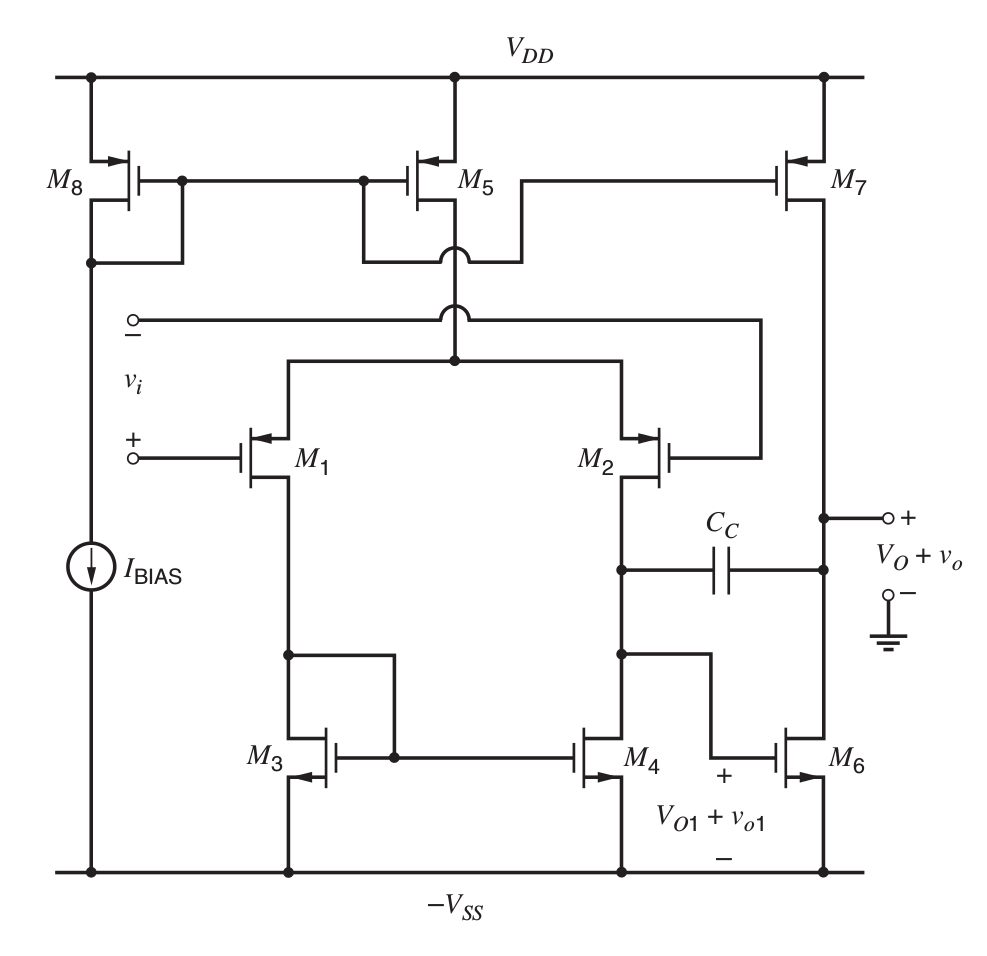
\includegraphics[scale=0.3]{./schem.png}
\end{center}
\end{figure}
\FloatBarrier
\begin{lstlisting}
OP-AMP
.OPTIONS LIST NODE POST
*.DC Vid -0.1 0.1 0.0001
*.OP
*.PRINT DC V(n4) V(n5) V(n7) I1(M1) I1(M2) PAR('V(n1)-V(n2)') I(R2) I1(M6)
.AC DEC 10 1 1E6
.parameter Vid = 0
.parameter Vic = 0
.parameter length = 0.25u

*****SUPPLIES

Vdd nvdd 0 DC 2V
Vss 0 nvss DC 2V
Ibias n6 nvss DC 10uA
*Itail nvdd n3 DC 100uA
*Ei1 n1 0 VOL = 'Vic + Vid'
*Ei2 n2 0 VOL = 'Vic - Vid'
Vi1 n1 0 DC 0
Vi2 n2 0 DC 0 AC 1

*****OP-AMP CORE - Figure 6-16 from book

C1 n5 n8 100p
R1 n8 n7 1626

M1 n4 n1 n3 nvdd CMOSP W = 50u L = length
M2 n5 n2 n3 nvdd CMOSP W = 50u L = length
M3 n4 n4 nvss nvss CMOSN W = 11.6u L = length
M4 n5 n4 nvss nvss CMOSN W = 11.6u L = length
M5 n3 n6 nvdd nvdd CMOSP W = 100u L = length
M6 n7 n5 nvss nvss CMOSN W = 11.6u L = length
M7 n7 n6 nvdd nvdd CMOSP W = 50u L = length

***** Self-Biasing current reference

M8 n6 n6 nvdd nvdd CMOSP W = 50u L = length
M9 n9 n6 nvdd nvdd CMOSP W = 50u L = length
M10 n6 n9 n10 nvss CMOSN W = 11.3u L = length
M11 n9 n10 nvss nvss CMOSN W = 11.3u L = length

R2 n10 nvss 50000

*****TRANSISTOR MODEL

.MODEL CMOSN NMOS (
+LEVEL   = 49             acm     = 3              hdif    = 0.35e-6
+VERSION = 3.1            TNOM    = 27             TOX     = 5.7E-9
+XJ      = 1E-7           NCH     = 2.3549E17      VTH0    = 0.4365497
+K1      = 0.3915623      K2      = 0.0175145      K3      = 1E-3
+K3B     = 2.6588343      W0      = 1E-7           NLX     = 1.111465E-7
+DVT0W   = 0              DVT1W   = 0              DVT2W   = 0
+DVT0    = -0.0408321     DVT1    = 0.0746768      DVT2    = 0.307109
+U0      = 407.1177485    UA      = 9.442714E-11   UB      = 1.092986E-18
+UC      = 1.63196E-11    VSAT    = 1.365087E5     A0      = 1.3189329
+AGS     = 0.2711719      B0      = 3.291713E-8    B1      = -1E-7
+KETA    = 4.645753E-3    A1      = 0              A2      = 1
+RDSW    = 439.9558234    PRWG    = 0.0345487      PRWB    = -0.0441065
+WR      = 1              WINT    = 1.645705E-9    LINT    = 1.116516E-9
+XL      = 3E-8           XW      = 0              DWG     = -1.494138E-9
+DWB     = 1.459097E-8    VOFF    = -0.1026054     NFACTOR = 0.1344887
+CIT     = 0              CDSC    = 1.527511E-3    CDSCD   = 0
+CDSCB   = 0              ETA0    = 1.930311E-3    ETAB    = 2.946158E-4
+DSUB    = 0.0214865      PCLM    = 1.3387947      PDIBLC1 = 0.480652
+PDIBLC2 = 9.034986E-3    PDIBLCB = -1E-3          DROUT   = 0.5593223
+PSCBE1  = 9.843289E9     PSCBE2  = 2.10878E-9     PVAG    = 1.0033136
+DELTA   = 0.01           MOBMOD  = 1              PRT     = 0
+UTE     = -1.5           KT1     = -0.11          KT1L    = 0
+KT2     = 0.022          UA1     = 4.31E-9        UB1     = -7.61E-18
+UC1     = -5.6E-11       AT      = 3.3E4          WL      = 0
+WLN     = 1              WW      = -1.22182E-16   WWN     = 1.2127
+WWL     = 0              LL      = 0              LLN     = 1
+LW      = 0              LWN     = 1              LWL     = 0
+CAPMOD  = 2              XPART   = 0.4            CGDO    = 3.11E-10
+CGSO    = 3.11E-10       CGBO    = 1E-11          CJ      = 1.758521E-3
+PB      = 0.99           MJ      = 0.457547       CJSW    = 4.085057E-10
+PBSW    = 0.8507757      MJSW    = 0.3374073      PVTH0   = 7.147521E-5
+PRDSW   = -67.2161633    PK2     = -1.344599E-3   WKETA   = 3.035972E-3
+LKETA   = -9.0406E-3     LAGS    = -0.3012         )
*
.MODEL CMOSP PMOS (
+LEVEL   = 49             acm     = 3              hdif    = 0.35e-6
+VERSION = 3.1            TNOM    = 27             TOX     = 5.7E-9
+XJ      = 1E-7           NCH     = 4.1589E17      VTH0    = -0.6586391
+K1      = 0.5199897      K2      = 0.0357513      K3      = 0
+K3B     = 15.5613889     W0      = 1E-6           NLX     = 1E-9
+DVT0W   = 0              DVT1W   = 0              DVT2W   = 0
+DVT0    = 2.6100181      DVT1    = 0.4363142      DVT2    = -0.042436
+U0      = 196.024903     UA      = 2.767112E-9    UB      = 1.90709E-18
+UC      = 6.166867E-11   VSAT    = 1.975064E5     A0      = 0.2398712
+AGS     = 0.0943234      B0      = 3.21184E-6     B1      = 5E-6
+KETA    = 0.0312217      A1      = 0              A2      = 1
+RDSW    = 997.072701     PRWG    = -0.1916111     PRWB    = -0.495
+WR      = 1              WINT    = 2.527293E-9    LINT    = 1.254514E-8
+XL      = 3E-8           XW      = 0              DWG     = -3.253948E-8
+DWB     = 4.92072E-8     VOFF    = -0.15          NFACTOR = 1.5460516
+CIT     = 0              CDSC    = 1.413317E-4    CDSCD   = 0
+CDSCB   = 0              ETA0    = 0.7241245      ETAB    = -0.240523
+DSUB    = 1.0813613      PCLM    = 2.0772083      PDIBLC1 = 4.31459E-4
+PDIBLC2 = 0.0252121      PDIBLCB = -9.960722E-4   DROUT   = 0.0432774
+PSCBE1  = 3.191047E10    PSCBE2  = 1.323218E-8    PVAG    = 0.0420525
+DELTA   = 0.01           MOBMOD  = 1              PRT     = 0
+UTE     = -1.5           KT1     = -0.11          KT1L    = 0
+KT2     = 0.022          UA1     = 4.31E-9        UB1     = -7.61E-18
+UC1     = -5.6E-11       AT      = 3.3E4          WL      = 0
+WLN     = 1              WW      = 0              WWN     = 1
+WWL     = 0              LL      = 0              LLN     = 1
+LW      = 0              LWN     = 1              LWL     = 0
+CAPMOD  = 2              XPART   = 0.4            CGDO    = 2.68E-10
+CGSO    = 2.68E-10       CGBO    = 1E-11          CJ      = 1.902493E-3
+PB      = 0.9810285      MJ      = 0.4644362      CJSW    = 3.142741E-10
+PBSW    = 0.9048624      MJSW    = 0.3304452      PVTH0   = 4.952976E-3
+PRDSW   = 29.8169373     PK2     = 3.383373E-3    WKETA   = -7.913501E-3
+LKETA   = -0.0208318      )
*
.end
\end{lstlisting}
\section{60 dB DC gain}
The first design objective for this lab was to obtain a 60 $\pm$ 3 dB of DC signal gain. The first step towards performing this was creating the spice netlist file for the OP-AMP given in figure 6.16 of Gray and Meyer. $(\frac{W}{l})$ for the transistors were initially based of a suggestion given in class by Prof. Higman of w = 10$\mu m$ for M3/M4 (assuming L = 0.25 $\mu m$ for all transistors). M1/M2 were sized W = 43$\mu m$ as the mobility of the p channel transistors are 4.3x smaller than the n channel ones, so by making the p-channel transistors longer they should have equivalent transconductance as the n channel ones. Finally M5 was set to twice M1/M3 as it carries twice the current, so W = 86. The biasing of the differential amplifier was initially chosen to arbitrarily 100$\mu A$, so M8 was set to 1/10 M5 to establish a mirror ratio to generate 100$\mu A$ (if the current of M8 is 10 microamps). Therefore the width of M8 was set to 8.6$\mu m$. Lastly, the output amplifier stage transisiters were matched to the diffamp transistor sizes to make the gain of each stage approximately the same. This design was then run in HSPICE, sweeping the input from -0.5 to 0.5 volts. Using a slope tool of Cosmoscope, the gain of this amplifer configuration was found to be approx. 550, or 54.8 dB, which was too low to meet the design requirement of 60 $\pm$ 3 dB. In order to increase the gain, the following derivation was made as an aid:
\begin{equation}
Av = g_m r_o = \sqrt{2i_dK_n^{'}\frac{W}{L}}\frac{Va}{i_d}= V_a\sqrt{\frac{2K_n^{'}\frac{W}{L}}{i_d}}
\end{equation}
Looking at this equation, we see that increasing the $(\frac{W}{l})$ and decreasing $i_d$ are both ways to increase the gain $A_v$. Therefore, first M5 was increased to 100$\mu m$ and all other transistors were resized using the same rationality as before. This yielded a gain increase to about 650, or 56.3 dB, still not quite enough. Finally, to increase gain again the size of the current in the opamp was decreased by increasing the current. Increasing M8 to W= 50$\mu m$ proved to be enough to get proper gain, bringing the diff-amp current to 20$\mu A$ and the second amplifier stage current to 10$\mu A$. The gain after doing this modification was about 750, or 57.5 dB, high enough to meet the design requirement. Below is a plot showing the input differential sweep against the output swing, with a slope measurement (representing gain).
\FloatBarrier
\begin{figure}[h!]
\begin{center}
 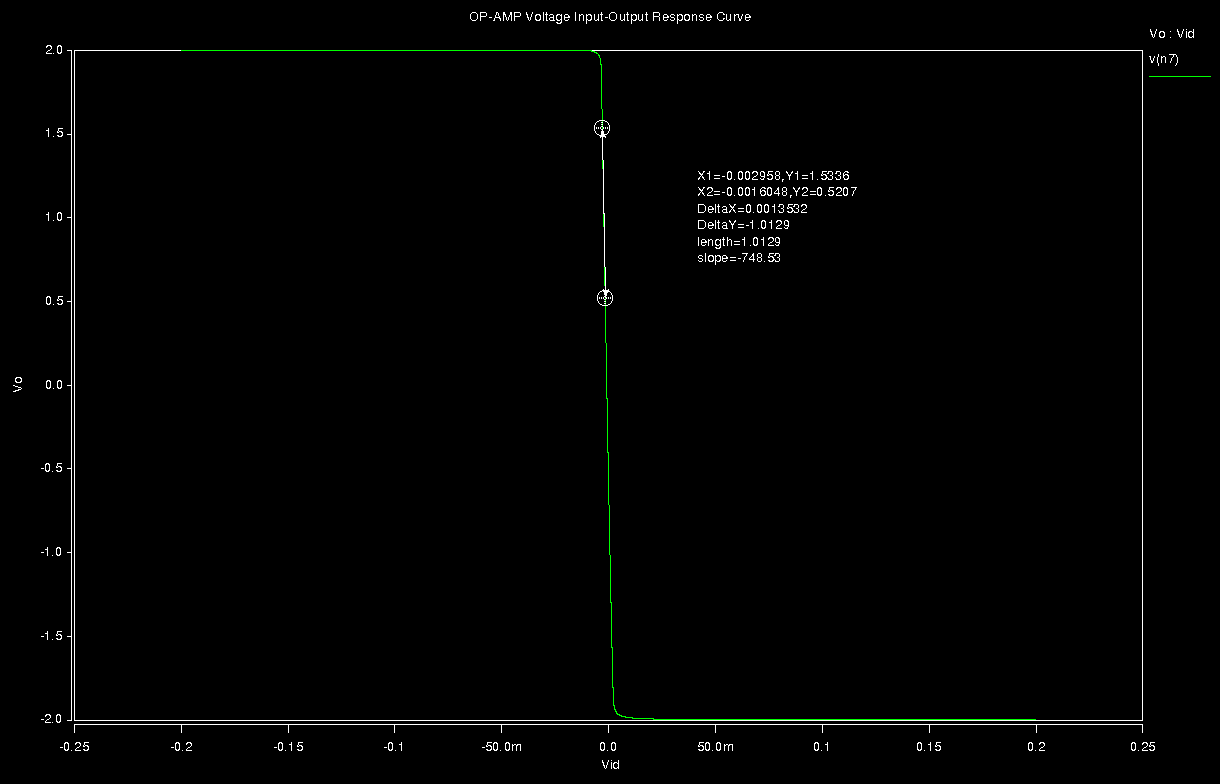
\includegraphics[scale=0.3]{./v-v.png}
\end{center}
\end{figure}
\FloatBarrier
\section{Power Supply Rejection}
The second task of the lab was to make sure the rejection of the biasing current to Vdd is less than 0.1.
Thus sensitivity is defined as:
\begin{equation}
S_{V_{dd}}^{i_o} = \frac{V_{dd}}{i_o}*\frac{\partial i_o}{\partial V_{dd}}
\end{equation}
A self-biasing current mirror constructed out of a current-mirror and a threshold-votlage referenced current reference was designed to achive the desired sensitivity. This current mirror was used to replace the ideal bias current in the OP-AMP schematic. Self-biasing current mirrors are known to have extremely low sensitivities as they will usually operate at one fixed point defined by the intersection of the input to output current curve of the mirror and the current reference. The design used took the form of the following schematic:
\FloatBarrier
\begin{figure}[h!]
\begin{center}
 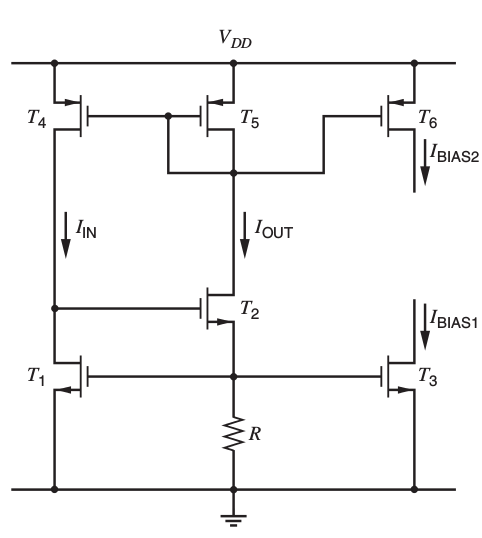
\includegraphics[scale=0.3]{./currf.png}
\end{center}
\end{figure}
\FloatBarrier
The P-channel transistors were matched to the size of M7 (50u) to ensure biasing of 10uA if the reference current is 10uA. The size of the R (R2 in netlist) was determined to be the value needed for a voltage drop of 0.5 volts, so 50k ohm. The threshold voltage of the n-channel FETS for the process used was determined to be 436 milivolts, meaning the overvoltage of the two N-FETS must be 64 millivolts for a 10uA bias current. Performing a simple calculation yielded that the widths of the two N-FETS must be 11.3um for 10uA bias current. This current refence was then build and the following simulation result was yielded:
\FloatBarrier
\begin{figure}[h!]
\begin{center}
 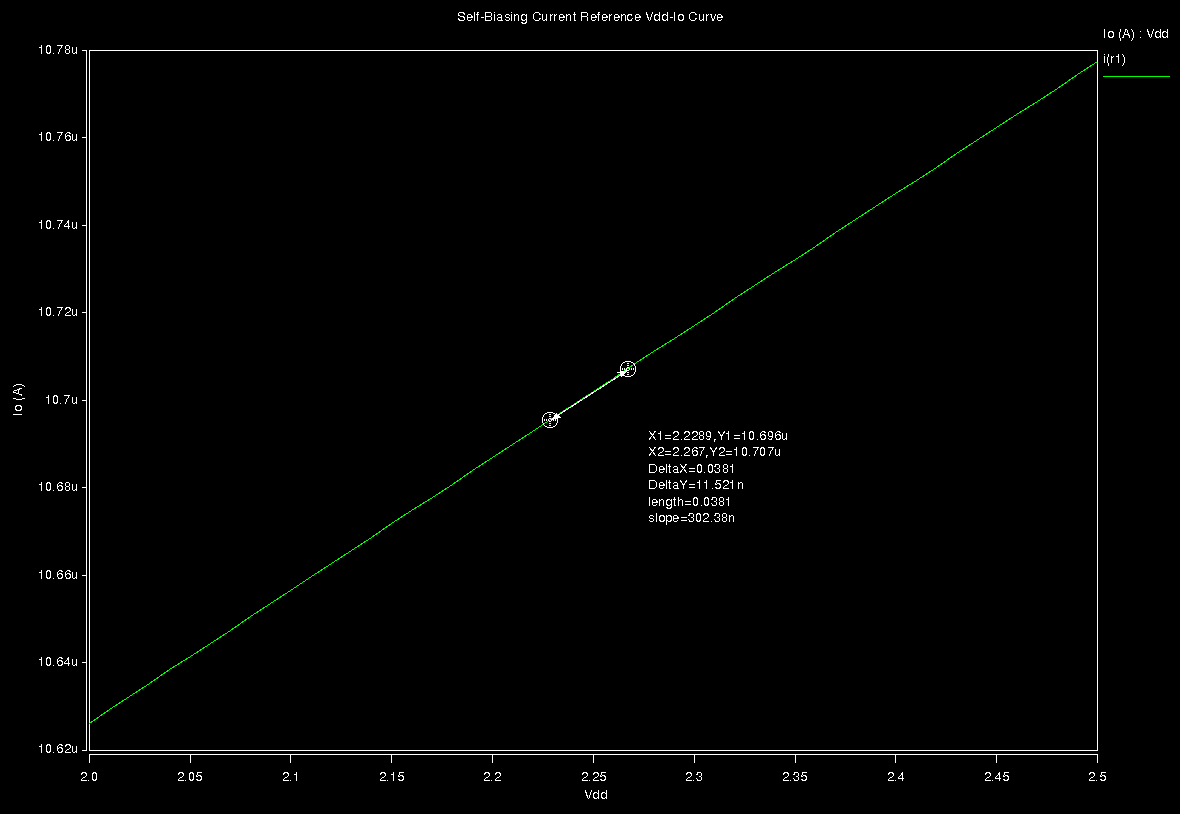
\includegraphics[scale=0.3]{./curr.png}
\end{center}
\end{figure}
\FloatBarrier
The current was very close to design, 10.62uA. The slope, ($\frac{\partial i_o}{\partial V_{dd}}$) was found to be 302nA/V, which gives a sensivitivy of
\begin{equation}
S_{V_{dd}}^{i_o} = \frac{2 V}{10.62\mu A}\times 302\frac{nA}{V} = 0.056
\end{equation}
This is less than the specification for 0.1.
\section{Compensation}
Below is the simulation for an AC sweep of the uncompensated OP-AMP designed in the previous parts. It has a pole neat 10 MHZ and likely not stable.
\FloatBarrier
\begin{figure}[h!]
\begin{center}
 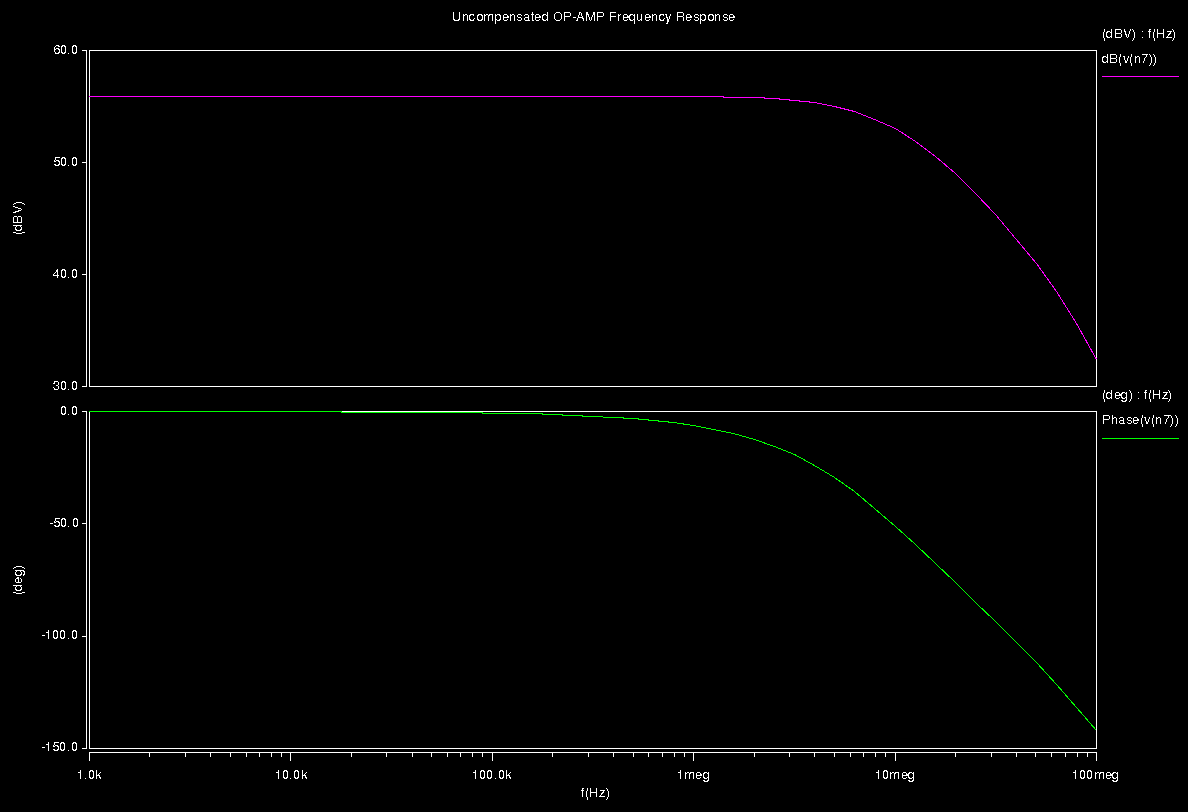
\includegraphics[scale=0.3]{./uncomp_f.png}
\end{center}
\end{figure}
\FloatBarrier

Below is the compensated opamp, using a compensation resistor of Rc = 1/gm6, as recommended by Prof. Higmann. It is unconditionally stable.

\FloatBarrier
\begin{figure}[h!]
\begin{center}
 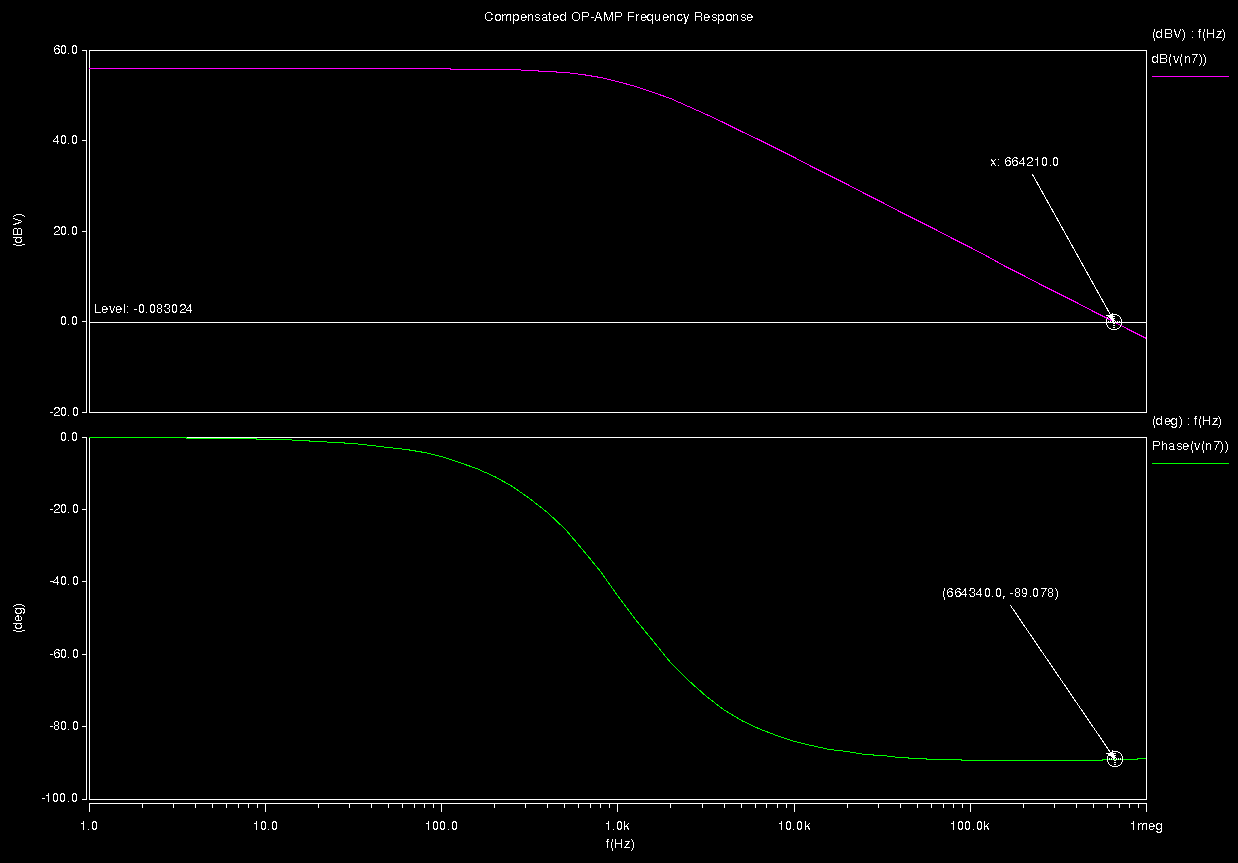
\includegraphics[scale=0.3]{./comp_f.png}
\end{center}
\end{figure}
\FloatBarrier

\section{Headroom}
To find the headroom of this amplifier, the OP-AMP was simply connected as a unity gain follower by connecting the output (n7) to the inverting input (n1) and then driving the non-inverting input with a swept DC source. The simulation for this yielded the below result, showing the headroom to essentially be rail to rail. More accurately, it was estimated to be between -1.956 and 1.994 volts, which is where the output becomes non-linear.
\FloatBarrier
\begin{figure}[h!]
\begin{center}
 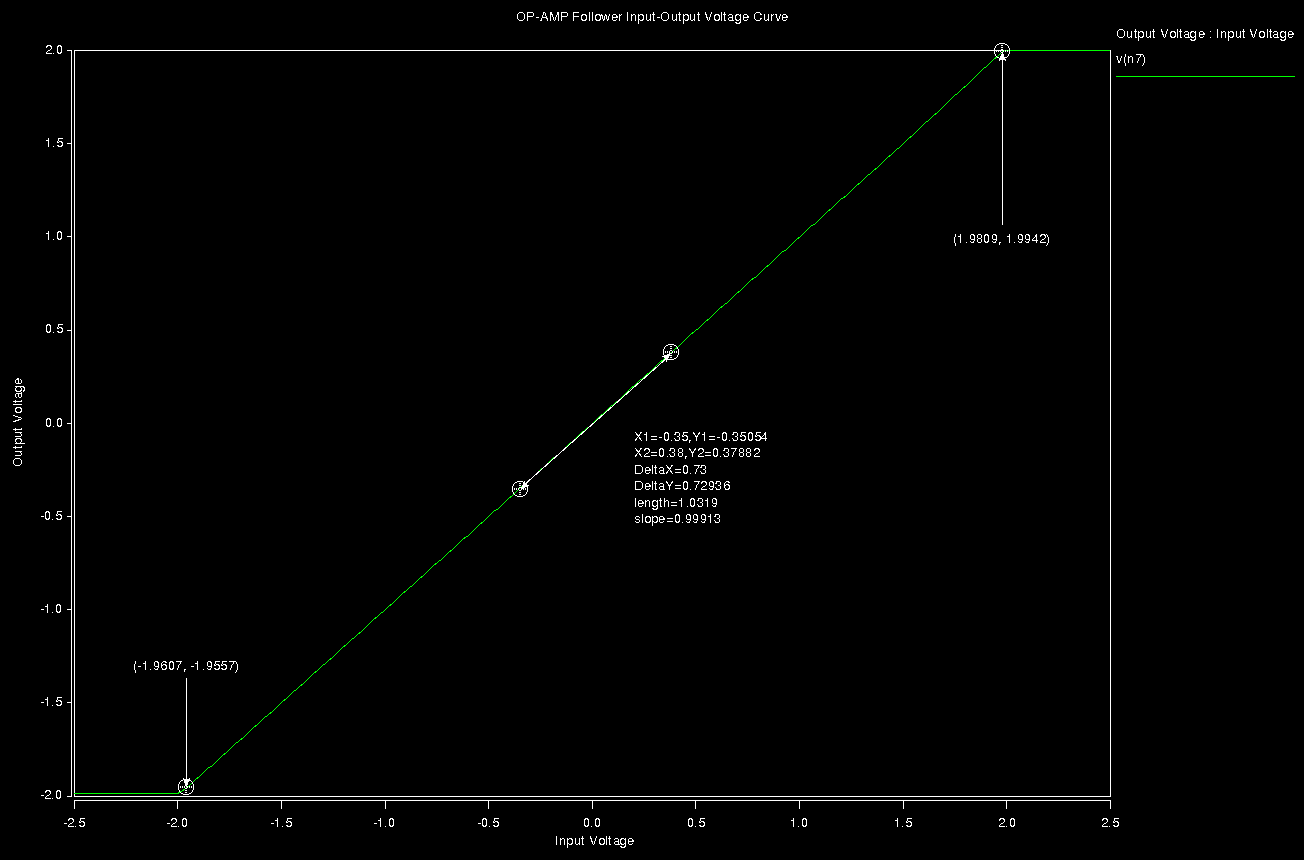
\includegraphics[scale=0.3]{./followerr.png}
\end{center}
\end{figure}
\FloatBarrier
\end{document}
